\chapter{Implementácia nástroja pre fuzzifikáciu numerických hodnôt} 
Nástroj má byť implementovaný v jazyku C++ a jeho výstupom má byť textový súbor s počtom centier a maticou fuzzifikovaných hodnôt. 

\section{Analýza a návrh}

Základná funkcionalita nástroja je spracovanie reálnych dát na fuzzy hodnoty. 
V kóde sa zadefinuje štruktúra dát a ako aj typ a počet výstupných atribútov. Následne pomocou metódy fuzzifikácie sa transformujú dané hodnoty na fuzzy hodnoty.  Návrh užívateľského rozhrania je konzolová aplikácia s preddefinovanou množinou dát a formátom. Vstupom budú dáta, ktoré budú v nadpriečinku Datasets v pričinku data a výstup sa zapíše v nadpriečinku Datasets do pričinka out. 


Pri analýze štruktúry programu som navrhla triedy Dataset, Fuzzification a štruktúru feature. Na obrázku číslo \ref{fig:pohlad} sú zobrazené spomínané triedy a ich vzťahy.





\begin{figure}[h]
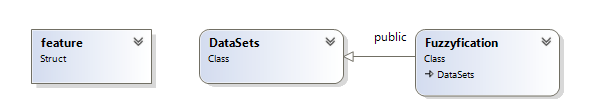
\includegraphics[width=0.75\textwidth]{obrazky/pohlad.PNG}
\centering
\caption{Návrh tried pre nástroj Fuzzy Tool} 
\label{fig:pohlad}
\end{figure}



\section{Implementácia nástroja fuzzy tool}

Nástroj bol implementovaný vo vývojom prostredí Visual Studio. Štruktúru projektu je  zobrazená na obrázku číslo \ref{fig:structure}.

\begin{figure}[h]
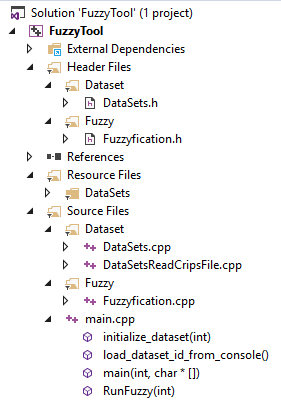
\includegraphics[]{obrazky/structure.PNG}
\centering
\caption{Štruktúra projektu pre nástroj Fuzzy Tool} 
\label{fig:structure}
\end{figure}


Na obrázku číslo \ref{diagramTried} je zobrazený diagram tried implementovaného fuzzy nástroja. Jednotlivé triedy a funkcionalitu opíšem v nasledujúcej časti. 


\subsection{Množiny dát - Datasets}
Štruktúra features slúži ako pomocná štuktúra pre triedu DataSets na zadefinovanie vstupných dát do vektoru reálnych hodnôt float Feature. DataSet predefinuje štruktúru vstupného typu dát, ktorá sa ďalej používa na fuzzifikáciu dát. Určí sa počet dát v datasete, počet atribútov (vlastností), vstupných a výstupných atribútov. Ďalej sú atribúty na počet výstupných intervalov datasetu, a ako aj počet lingvistických (nie numerických) atribútov, názov datasetu, a vektor vzoru štruktúry feature. Medzi najhlavnejšie metódy patrí čítanie dát zo súboru, normovnaie dát, a zápis čistých dát do súboru, a vypočítanie počiatočnej chyby dát. Medzi pomocné metódy triedy patrí získanie dát zo súboru, načítanie konkrétneho datasetu podľa zadefinovanej štruktúry dát, a inicializácia atribútov. 
\subsubsection{Spracovanie dát}
Inicializácia dát sa vykonavá podľa vopred zadefinovaného identifikačného čísla datasetu, a následne sa zadefinuje počet dát v datasete, vstupných, vystupných atribútov a počet výstupných intervalov. 

Načítanie dát daného datasetu zo súboru sa vykonáva pomocou metódy ReadDataSets, ktorá používa metódu get\_dataset\_file. 
Metóda podľa identifikačného čísla vykoná danú metódu, kde je definované načítavanie konkrétnej množiny dát podľa zadaného formatovacieho výrazu. 

Dáta sa znormalizujú podľa minimálnej a maximálnej hodnoty atribútu v danej vlastnosti (feature) do intervalu $<0,1>$. 

\subsection{Fuzzifikácia hodnôt}
Metódou RunFuzzification sa spustí celý proces fuzzifikovania dát. Pre lepšiu čitateľnosť a orientáciu v kóde boli  jednotlivé podčasti algoritmu rozdelené do osobitných súkromných metód. 


Metóda ktorá robí hlavný výpočet obsahuje nasledovné podčasti: 
\begin{itemize}
\item inicializácia normalizovnaného datasetu, 
\item inicializácia premenných a vektorov, 
\item vytvorenie features pre počiatočný interval 2, 
\item v cykle prejdem všetky rozmery vstupných atribútov
\begin{itemize}
\item inicializujem hodnoty pre novú entropiu, 
\item ak sa entorpia zmenila, tak modifikujem rozmer features, 
\item určím počet intervalov, 
\item lokalizujem centrum intervalov, 
\begin{itemize}
\item určenie počtu klastrov, 
\item určenie centra klastrov, 
\item označenie klastra každého elementu, 
\item prepočítanie centier klastrov, 
\end{itemize}
\item určím funkciu príslušnosti pomocou FCM algoritmu, 
\item vypočítam celkovú váženú fuzzy entorpiu pre intervaly I a I-1
\begin{itemize}
\item nastavím univerzánu množinu X,
\item nastavím fuzzy množinu obsahujúcu k elementov,
\item nastavím vektor reprezentujúci m tried do ktorých bude rozdelených n elementov, 
\item nastavím množinu scj ako množinu elementov reprezentujúcu triedu j na množine X, 
\item vypočítam stupeň príslušnosti $D_j$ pomocu váženého priemeru, 
\item vypočítam fuzzy entropiu fecj A,
\item vypočítam fuzzy entropiu FEA na X množine
\end{itemize}

\item v nekonečnom cykle kontrolujem podmienku, ak sa entropia zníži, tak sa skončím cyklus, 
\end{itemize}
\item vypíšem výsledky do súboru. 
\end{itemize}

\section{Main trieda}
V main načítavam vstup od používateľa - číslo datasetu a dáta. Následne sa spustí fuzzifikácia a užívateľovi sú ukázané priebežný priebeh výpočtu. Po skončení výpočtu sú zapísané dáta do súboru a pomocné výpočty do logovacieho súboru. 

Na obrázku č.\ref{fig:consola} je zobrazená ukážka konzolovej aplikácie, na obrázku č. \ref{fig:vysledky} výsledky fuzzifikácie daného datasetu, a na obrázku č. \ref{fig:logSubor} zobrazené priebežné výsledky fuzzifikácie. 

\begin{figure}[h]
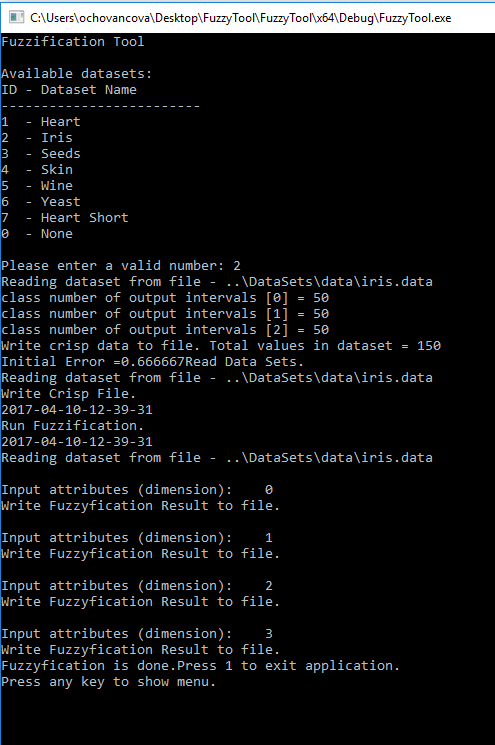
\includegraphics{obrazky/consola1.PNG}
\centering
\caption{Ukážka konzolovej aplikácie nástroja Fuzzy Tool} 
\label{fig:consola}
\end{figure}

\begin{figure}[h]
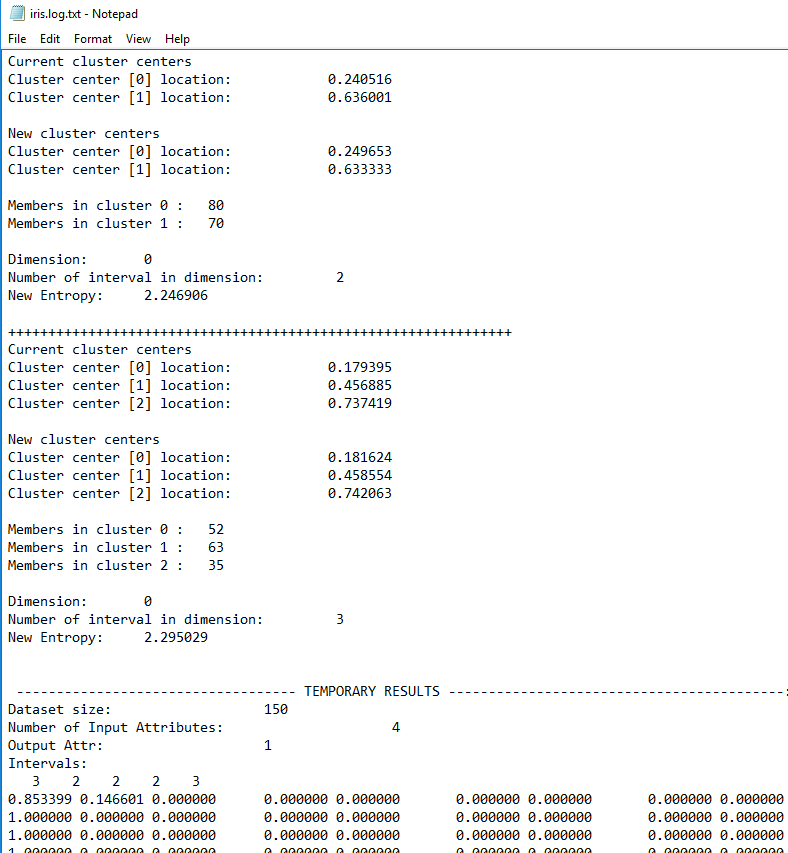
\includegraphics[width=0.85\textwidth]{obrazky/logSubor.PNG}
\centering
\caption{Ukážka výstupu logovací súbor nástroja Fuzzy Tool} 
\label{fig:logSubor}
\end{figure}

\begin{figure}[h]
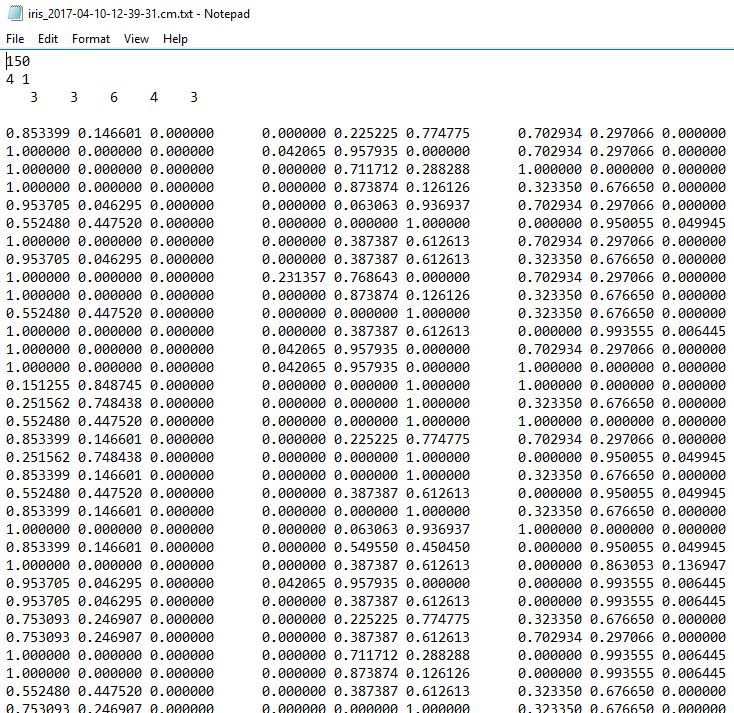
\includegraphics[width=0.85\textwidth]{obrazky/vysledkySubor.PNG}
\centering
\caption{Ukážka výstupu výsledkov fuzzifikácie nástroja Fuzzy Tool} 
\label{fig:vysledky}
\end{figure}

